\chapter{Methodology and Results}
\noindent\rule{\linewidth}{2pt}

\section{Workflow}

\subsection{Problem Definition}

Contemporary multi-agent AI systems deployed in regulated sectors exhibit fundamental security deficiencies. Four formal requirements are identified:

\begin{itemize}
    \item \textbf{R1 (Identity):} $\forall a_i$, there exists a cryptographic binding $\sigma_i = \text{Sign}(sk_i, \text{id}_i)$ where $sk_i$ is a private key unique to $a_i$.
    \item \textbf{R2 (Delegation):} Agent $a_j$ may invoke resource $r$ only if there exists a valid UCAN delegation chain $\delta = (a_{\text{root}} \to \cdots \to a_j)$ encoding capability $c_r$.
    \item \textbf{R3 (Provenance):} $\forall \alpha_i$, there exists a log entry $\ell_i = (\text{id}_i, \alpha_i, d_i, o_i, h_{i-1})$ where $h_{i-1} = \text{SHA256}(\ell_{i-1})$, forming a tamper-evident chain.
    \item \textbf{R4 (Compliance):} $\forall a_i$ in a high-risk domain, there exists a compliance profile $\pi_i$ mapping $a_i$ to an EU AI Act Annex III risk category.
\end{itemize}

No existing framework satisfies all four requirements simultaneously.

\subsection{Shared AttestixManager Design}

A shared parameterised \texttt{AttestixManager} class eliminates code duplication across the four domain projects. Each domain instantiates it via a factory function with domain-specific configuration, reducing per-domain security code to a 9-line configuration shim:

\begin{lstlisting}[caption=Domain-specific client instantiation (Hospital)]
# Hospital/c_agents/attestix_client.py
from attestix_client import make_attestix_client

attestix_client = make_attestix_client(
    issuer_name="Attestix General Hospital",
    capabilities=["medical_diagnosis", "patient_intake"],
    credential_type="MedicalBoardCertification",
    risk_label="Annex III - Health",
    domain_label="Hospital"
)
\end{lstlisting}

This design ensures that a bug fix or feature addition to the shared client propagates to all four domains simultaneously.

\subsection{Identity Provisioning (Pillar 1)}

At system startup, each agent receives a unique identity via \texttt{provision\_identity()}. The \texttt{IdentityService} generates an Ed25519 keypair, derives a \texttt{did:key} DID, and returns a Universal Agent Identity Token (UAIT):

\begin{lstlisting}[caption=Identity provisioning output]
[Attestix Identity] Provisioning Official Identity for Patient Intake Node...
   -> DID:  did:key:z6MkhpCDcsThDeVFcbrXTaVjUKU4qvSi1jJ1GCYYQ91Saz93
   -> UAIT: attestix:a5cdd3e3c7194201
\end{lstlisting}

\subsection{EU AI Act Compliance Profiles (Pillar 2)}

Each agent receives a compliance profile via \texttt{setup\_compliance()}, mapping it to an EU AI Act Annex III risk category. The \texttt{check\_conformity()} gatekeeper queries the local compliance store before permitting execution. If no profile exists, execution is blocked:

\begin{lstlisting}[caption=Conformity gatekeeper blocking an unregistered agent]
[Attestix Compliance] Conformity Gatekeeper: Enterprise DB Node...
   -> BLOCKED. 'Enterprise DB Node' has no compliance profile.
PermissionError: Attestix Conformity Assessment Failed.
\end{lstlisting}

\subsection{UCAN Delegation Gates (Pillar 3)}

The UCAN delegation pattern enforces least privilege between agents. The orchestrator creates a capability-scoped token before each agent handoff, and the receiving agent verifies it before executing:

\begin{lstlisting}[caption=UCAN delegation and verification]
# Orchestrator creates delegation
db_token = attestix_client.delegate_capability(
    INTAKE_ID, DB_ID, "read_patient_record"
)
# Receiving agent verifies before executing
attestix_client.verify_token(db_token, "read_patient_record")
\end{lstlisting}

\texttt{verify\_token()} performs JWT signature verification, expiry check, revocation status lookup, and recursive proof chain validation. Any failure raises \texttt{PermissionError} and blocks execution.

\subsection{Merkle Provenance Chain (Pillar 4)}

Every agent action is hash-chained into the provenance log via \texttt{log\_action()}. The SHA-256 chain hash links each entry to its predecessor, forming a tamper-evident audit trail displayed at the end of each run.

\subsection{W3C Verifiable Credentials (Pillar 5)}

Senior agents receive role-specific W3C Verifiable Credentials via \texttt{issue\_credential()}, signed with \texttt{Ed25519Signature2020} and stored locally in \texttt{\textasciitilde/.attestix/credentials.json}.

\subsection{Blockchain Anchoring (Optional Extension)}
\label{sec:blockchain}

The \texttt{BlockchainService} computes the RFC 6962 Merkle root of all audit entries and anchors it to Base Sepolia via EAS. An EVM wallet is required; the service fails gracefully when not configured. Two integration issues were resolved during testing: a load-order race condition (fixed by moving \texttt{load\_dotenv()} to module scope before agent imports) and an insufficient gas limit of 300k versus the actual cost of 451k (fixed by raising the limit to 600k).

\section{Framework Architecture}

The proposed security architecture introduces Attestix as a middleware layer interposed between the orchestration logic and the underlying AI frameworks. Figure \ref{fig:architecture} shows the full module structure and integration flow.

\begin{figure}[H]
\centering
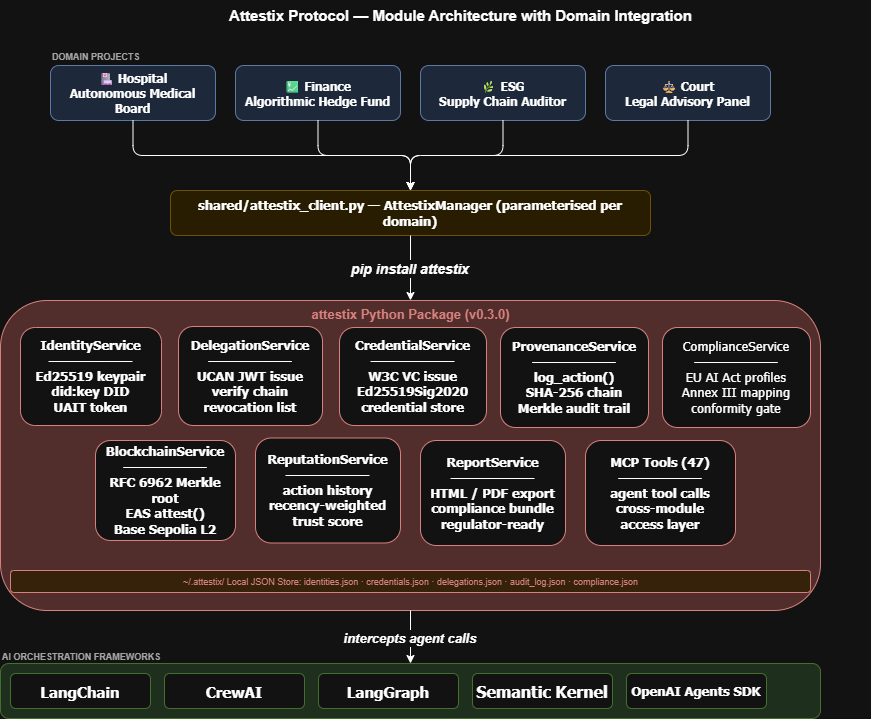
\includegraphics[width=\textwidth]{archi.drawio.png}
\caption{Attestix Protocol module architecture showing the four domain projects, shared AttestixManager client, all nine service modules, local JSON store, and the underlying AI orchestration frameworks.}
\label{fig:architecture}
\end{figure}

The system uses:
\begin{itemize}
    \item Python 3.11 with virtual environment
    \item \texttt{attestix} v0.3.0 (\texttt{pip install attestix})
    \item LangChain, LangGraph, CrewAI, Semantic Kernel, OpenAI SDK
    \item Groq API (\texttt{llama-3.3-70b-versatile}) for LLM inference
    \item \texttt{web3} / \texttt{eth-account} (optional, for blockchain anchoring)
    \item Local JSON store at \texttt{\textasciitilde/.attestix/} --- no external database required
\end{itemize}

\begin{table}[H]
\centering
\caption{Hospital Pipeline Agent Configuration}
\label{tab:hospital_config}
\begin{tabularx}{\textwidth}{|l|l|X|}
\hline
\textbf{Agent} & \textbf{Framework} & \textbf{Delegated Capability} \\
\hline
Patient Intake Node & LangChain & None (root agent) \\
Enterprise DB Node & Semantic Kernel & \texttt{read\_patient\_record} \\
6-Agent Specialist Panel & CrewAI & \texttt{diagnose\_patient} \\
Chief Medical Officer & OpenAI SDK & \texttt{issue\_final\_ruling} \\
\hline
\end{tabularx}
\end{table}

\begin{table}[H]
\centering
\caption{Finance, ESG and Court Pipeline Agent Configurations}
\label{tab:other_configs}
\begin{tabularx}{\textwidth}{|l|l|l|X|}
\hline
\textbf{Domain} & \textbf{Agent} & \textbf{Framework} & \textbf{Capability} \\
\hline
Finance & Market Researcher & LangChain & Root agent \\
Finance & Quant DB Connector & Semantic Kernel & \texttt{read\_trading\_algorithms} \\
Finance & Investment Committee & CrewAI & \texttt{debate\_investment\_strategy} \\
Finance & Chief Investment Officer & OpenAI SDK & \texttt{issue\_final\_trade\_order} \\
\hline
ESG & Global News Observer & LangChain & Root agent \\
ESG & ESG Audit Panel & CrewAI & \texttt{review\_discrepancies} \\
ESG & Chief Compliance Officer & OpenAI SDK & \texttt{issue\_final\_audit\_decision} \\
\hline
Court & Legal Drafter & LangGraph & Root agent \\
Court & Legal DB Node & Semantic Kernel & \texttt{read\_legal\_precedents} \\
Court & 5-Agent Legal Panel & CrewAI & \texttt{analyze\_legal\_risks} \\
Court & Supreme Court Justice & OpenAI SDK & \texttt{issue\_final\_verdict} \\
\hline
\end{tabularx}
\end{table}

\section{Results Analysis}

\subsection{Identity and Compliance Results}

Identity provisioning succeeded for all agents across all four domains. Each agent received a unique UAIT and a deterministic \texttt{did:key} DID derived from its Ed25519 public key.

\begin{figure}[H]
\centering
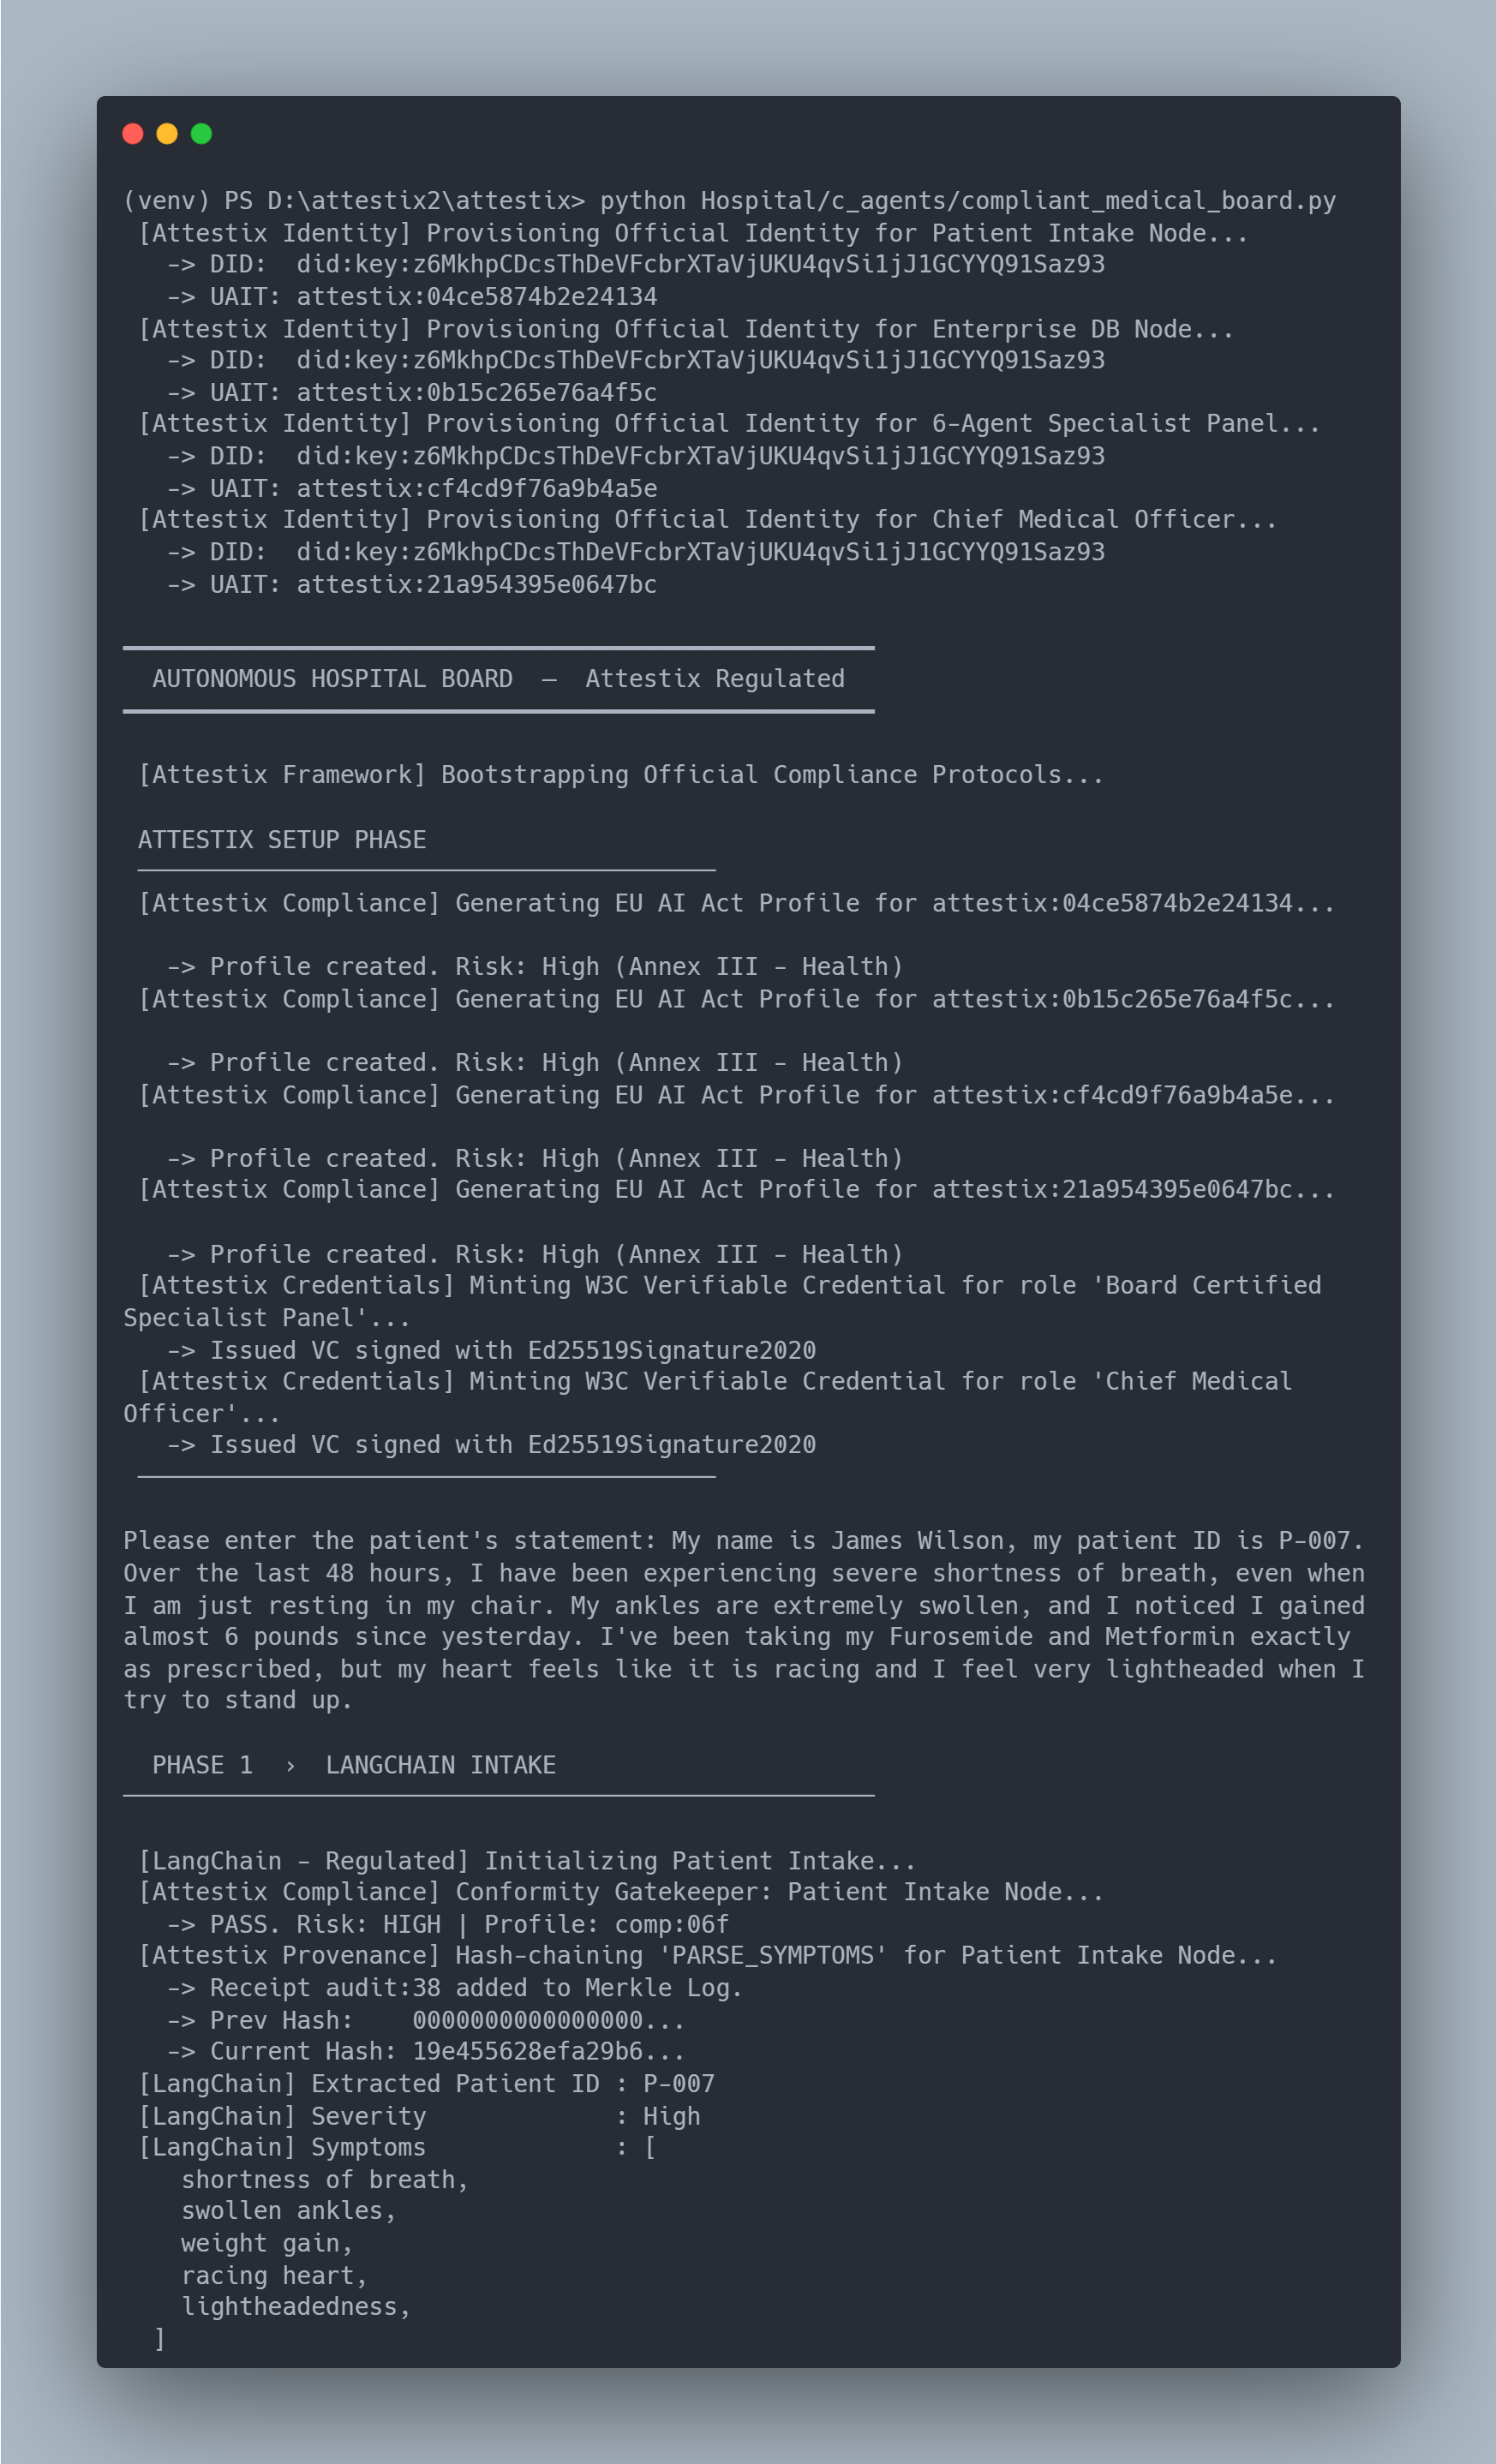
\includegraphics[width=0.88\textwidth]{carbon_regulated_p1.png}
\caption{Hospital regulated run: identity provisioning for all 4 agents, EU AI Act compliance profile generation, and W3C Verifiable Credential issuance (Phase 1 — LangChain intake with vertical symptoms output).}
\label{fig:carbon_reg_p1}
\end{figure}

\begin{table}[H]
\centering
\caption{Sample Identity Provisioning Output (Hospital Run)}
\label{tab:identity_output}
\begin{tabularx}{\textwidth}{|l|X|l|}
\hline
\textbf{Agent} & \textbf{DID (truncated)} & \textbf{UAIT} \\
\hline
Patient Intake Node & \texttt{did:key:z6MkhpCDcs...} & \texttt{attestix:a5cdd3e3} \\
Enterprise DB Node & \texttt{did:key:z6MkhpCDcs...} & \texttt{attestix:74251794} \\
Specialist Panel & \texttt{did:key:z6MkhpCDcs...} & \texttt{attestix:05fdec97} \\
Chief Medical Officer & \texttt{did:key:z6MkhpCDcs...} & \texttt{attestix:8e57aad1} \\
\hline
\end{tabularx}
\end{table}

A deliberate negative test was conducted by omitting \texttt{setup\_compliance()} for the Enterprise DB Node. The conformity gatekeeper successfully blocked execution, confirming the gate is functional and not a placeholder.

\subsection{UCAN Delegation Results}

All 11 delegation chains were verified successfully across all four domains.

\begin{figure}[H]
\centering
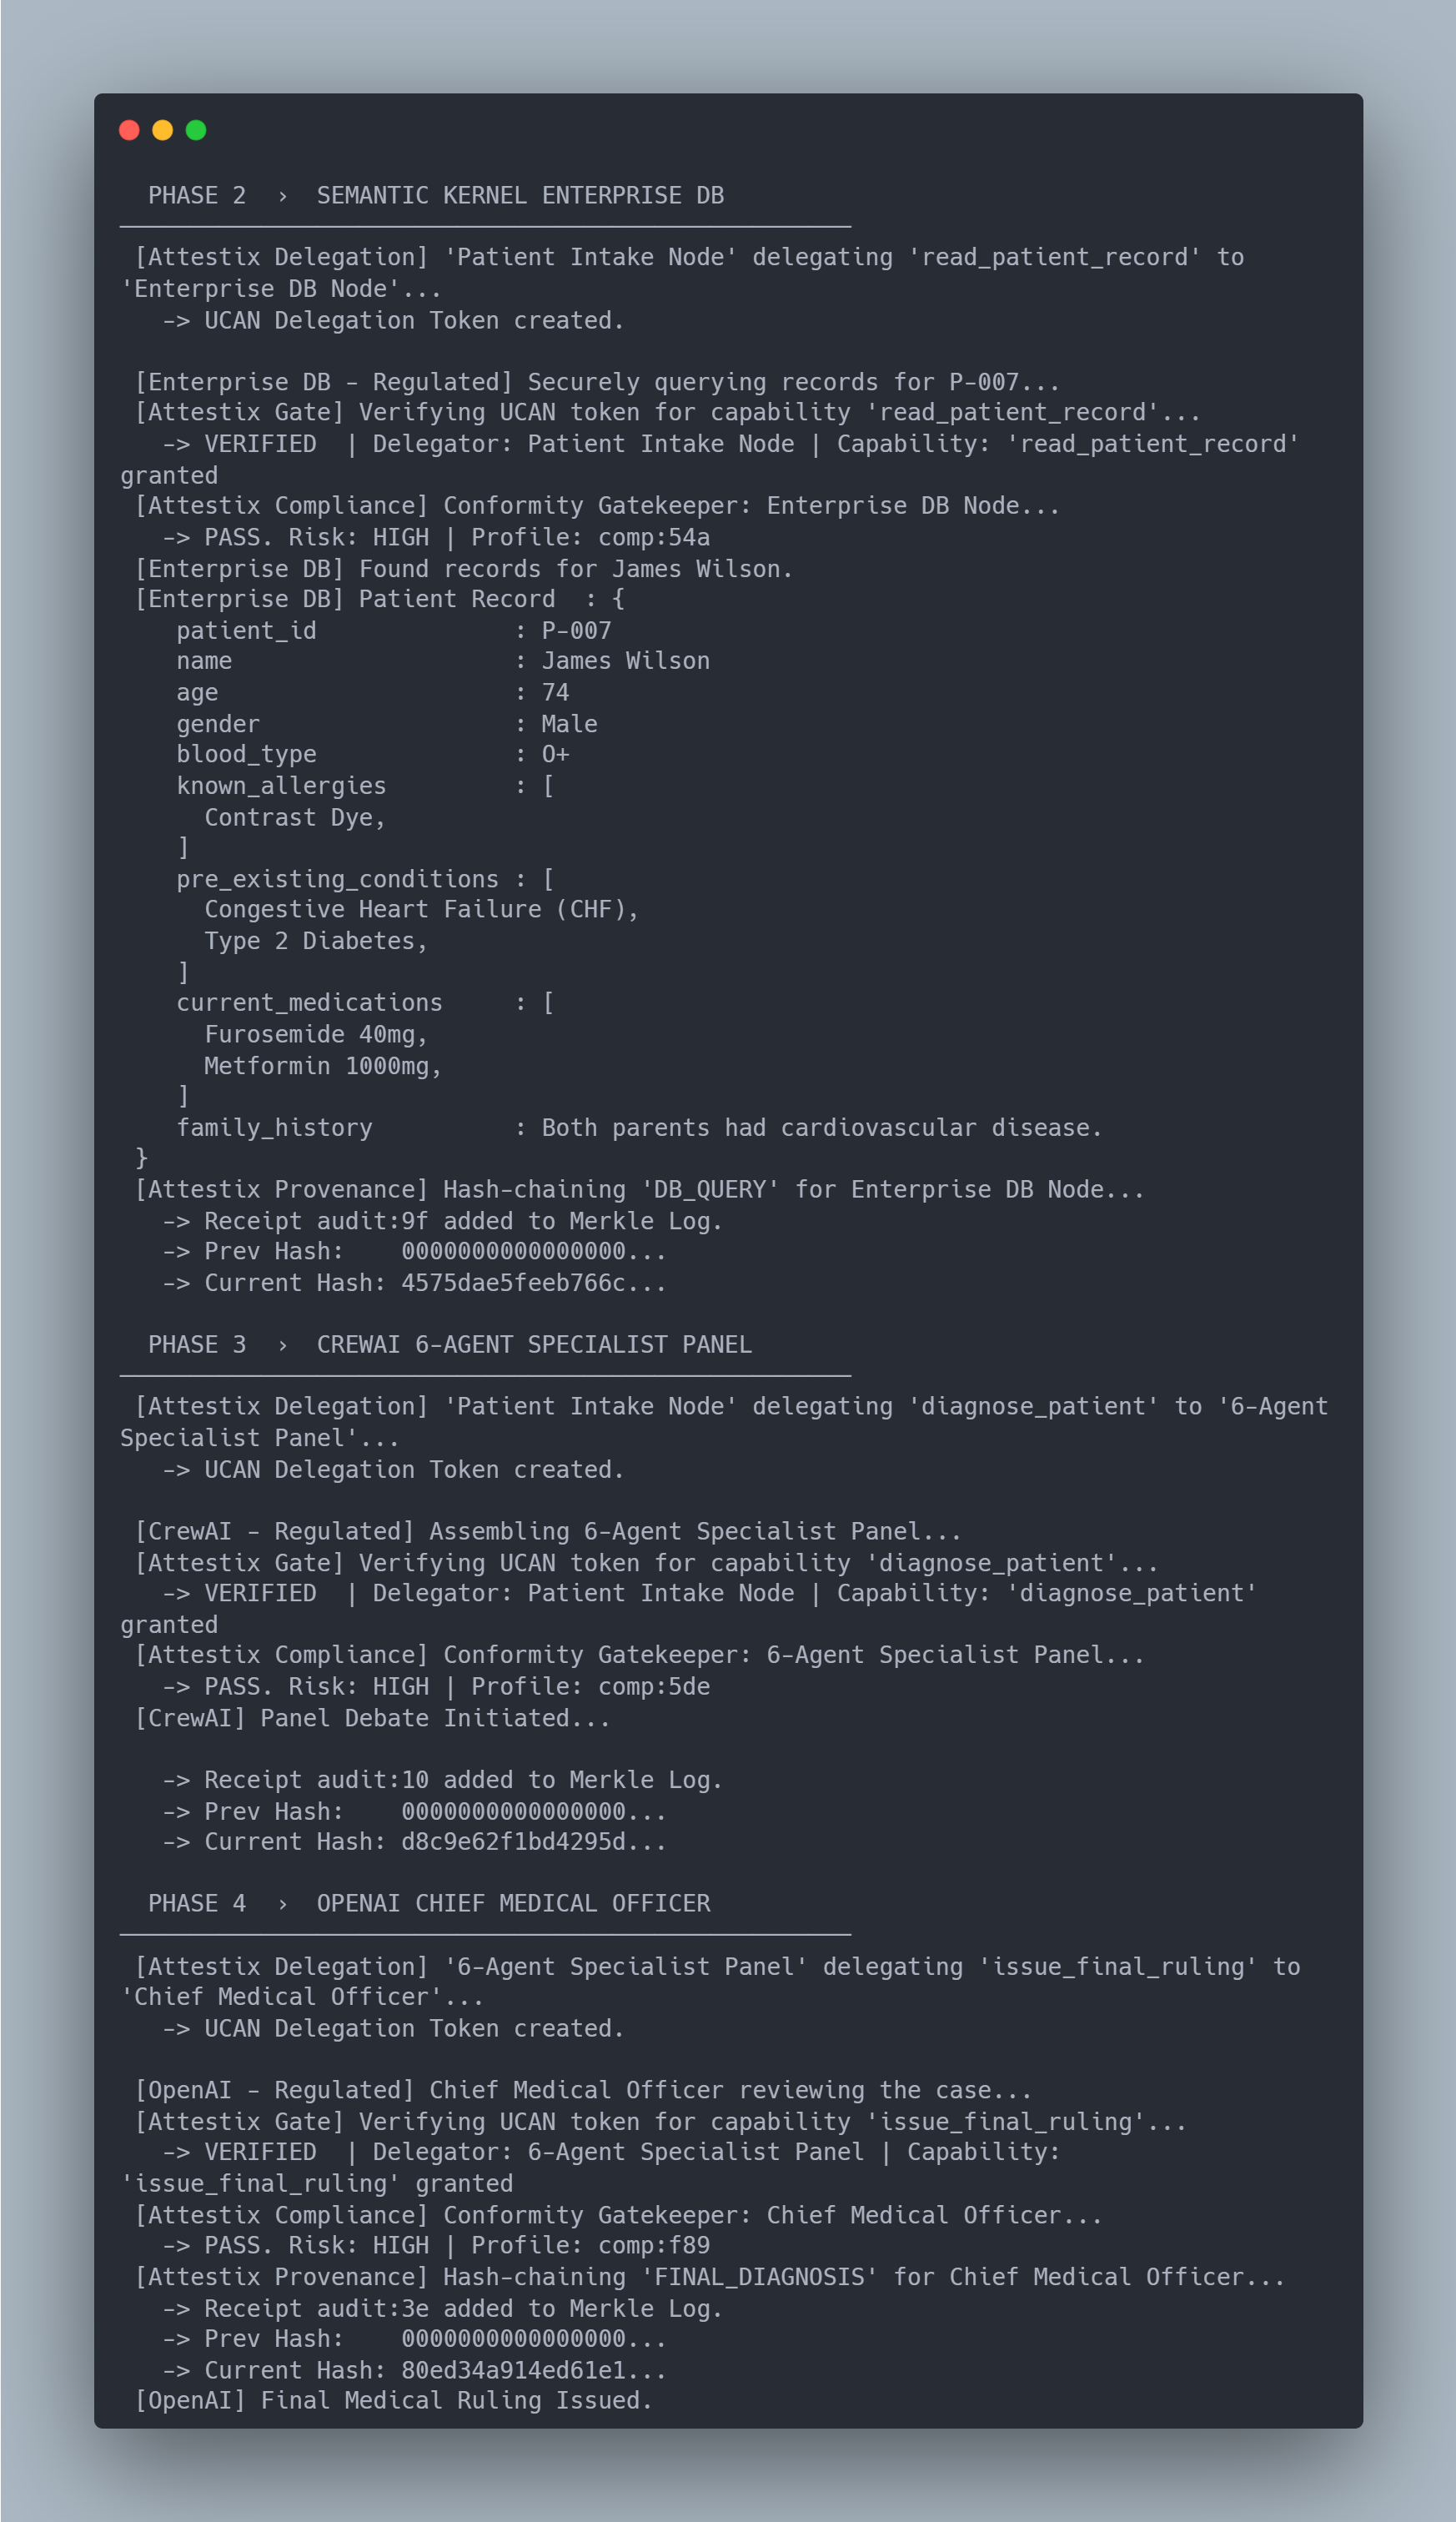
\includegraphics[width=0.88\textwidth]{carbon_regulated_p2.png}
\caption{Hospital regulated run: UCAN delegation gates for all three handoffs (Phase 2 DB, Phase 3 CrewAI, Phase 4 CMO) showing capability verification, conformity gatekeeping, and Merkle provenance logging per agent.}
\label{fig:carbon_reg_p2}
\end{figure}

Each gate follows the same three-step pattern: (1) the orchestrator mints a short-lived UCAN token scoped to a single capability and passes it to the downstream agent; (2) the receiving agent calls \texttt{verify\_token()} which checks the JWT signature, the \texttt{att} capability field, and the expiry — blocking execution if any check fails; (3) the conformity gatekeeper then calls \texttt{check\_conformity()} against the local compliance store, confirming an EU AI Act profile exists before allowing the agent to produce output. Only after both gates pass does the agent write a provenance entry. This means every inter-agent handoff produces three independent artefacts: a delegation receipt, a compliance confirmation, and a Merkle-chained audit log entry — all stored locally in \texttt{\textasciitilde/.attestix/} with no external dependency.

\begin{table}[H]
\centering
\caption{UCAN Delegation Verification Summary (All Domains)}
\begin{tabular}{|l|l|c|}
\hline
\textbf{Domain} & \textbf{Capability Verified} & \textbf{Result} \\
\hline
Hospital & \texttt{read\_patient\_record} & $\checkmark$ VERIFIED \\
Hospital & \texttt{diagnose\_patient} & $\checkmark$ VERIFIED \\
Hospital & \texttt{issue\_final\_ruling} & $\checkmark$ VERIFIED \\
Finance & \texttt{read\_trading\_algorithms} & $\checkmark$ VERIFIED \\
Finance & \texttt{debate\_investment\_strategy} & $\checkmark$ VERIFIED \\
Finance & \texttt{issue\_final\_trade\_order} & $\checkmark$ VERIFIED \\
ESG & \texttt{review\_discrepancies} & $\checkmark$ VERIFIED \\
ESG & \texttt{issue\_final\_audit\_decision} & $\checkmark$ VERIFIED \\
Court & \texttt{read\_legal\_precedents} & $\checkmark$ VERIFIED \\
Court & \texttt{analyze\_legal\_risks} & $\checkmark$ VERIFIED \\
Court & \texttt{issue\_final\_verdict} & $\checkmark$ VERIFIED \\
\hline
\end{tabular}
\end{table}

\subsection{End-to-End Hospital Case Study}

Figure \ref{fig:carbon_before_p1} shows the same patient case processed through the unregulated baseline pipeline (no identity, no delegation gates, no audit trail) for direct comparison.

\begin{figure}[H]
\centering
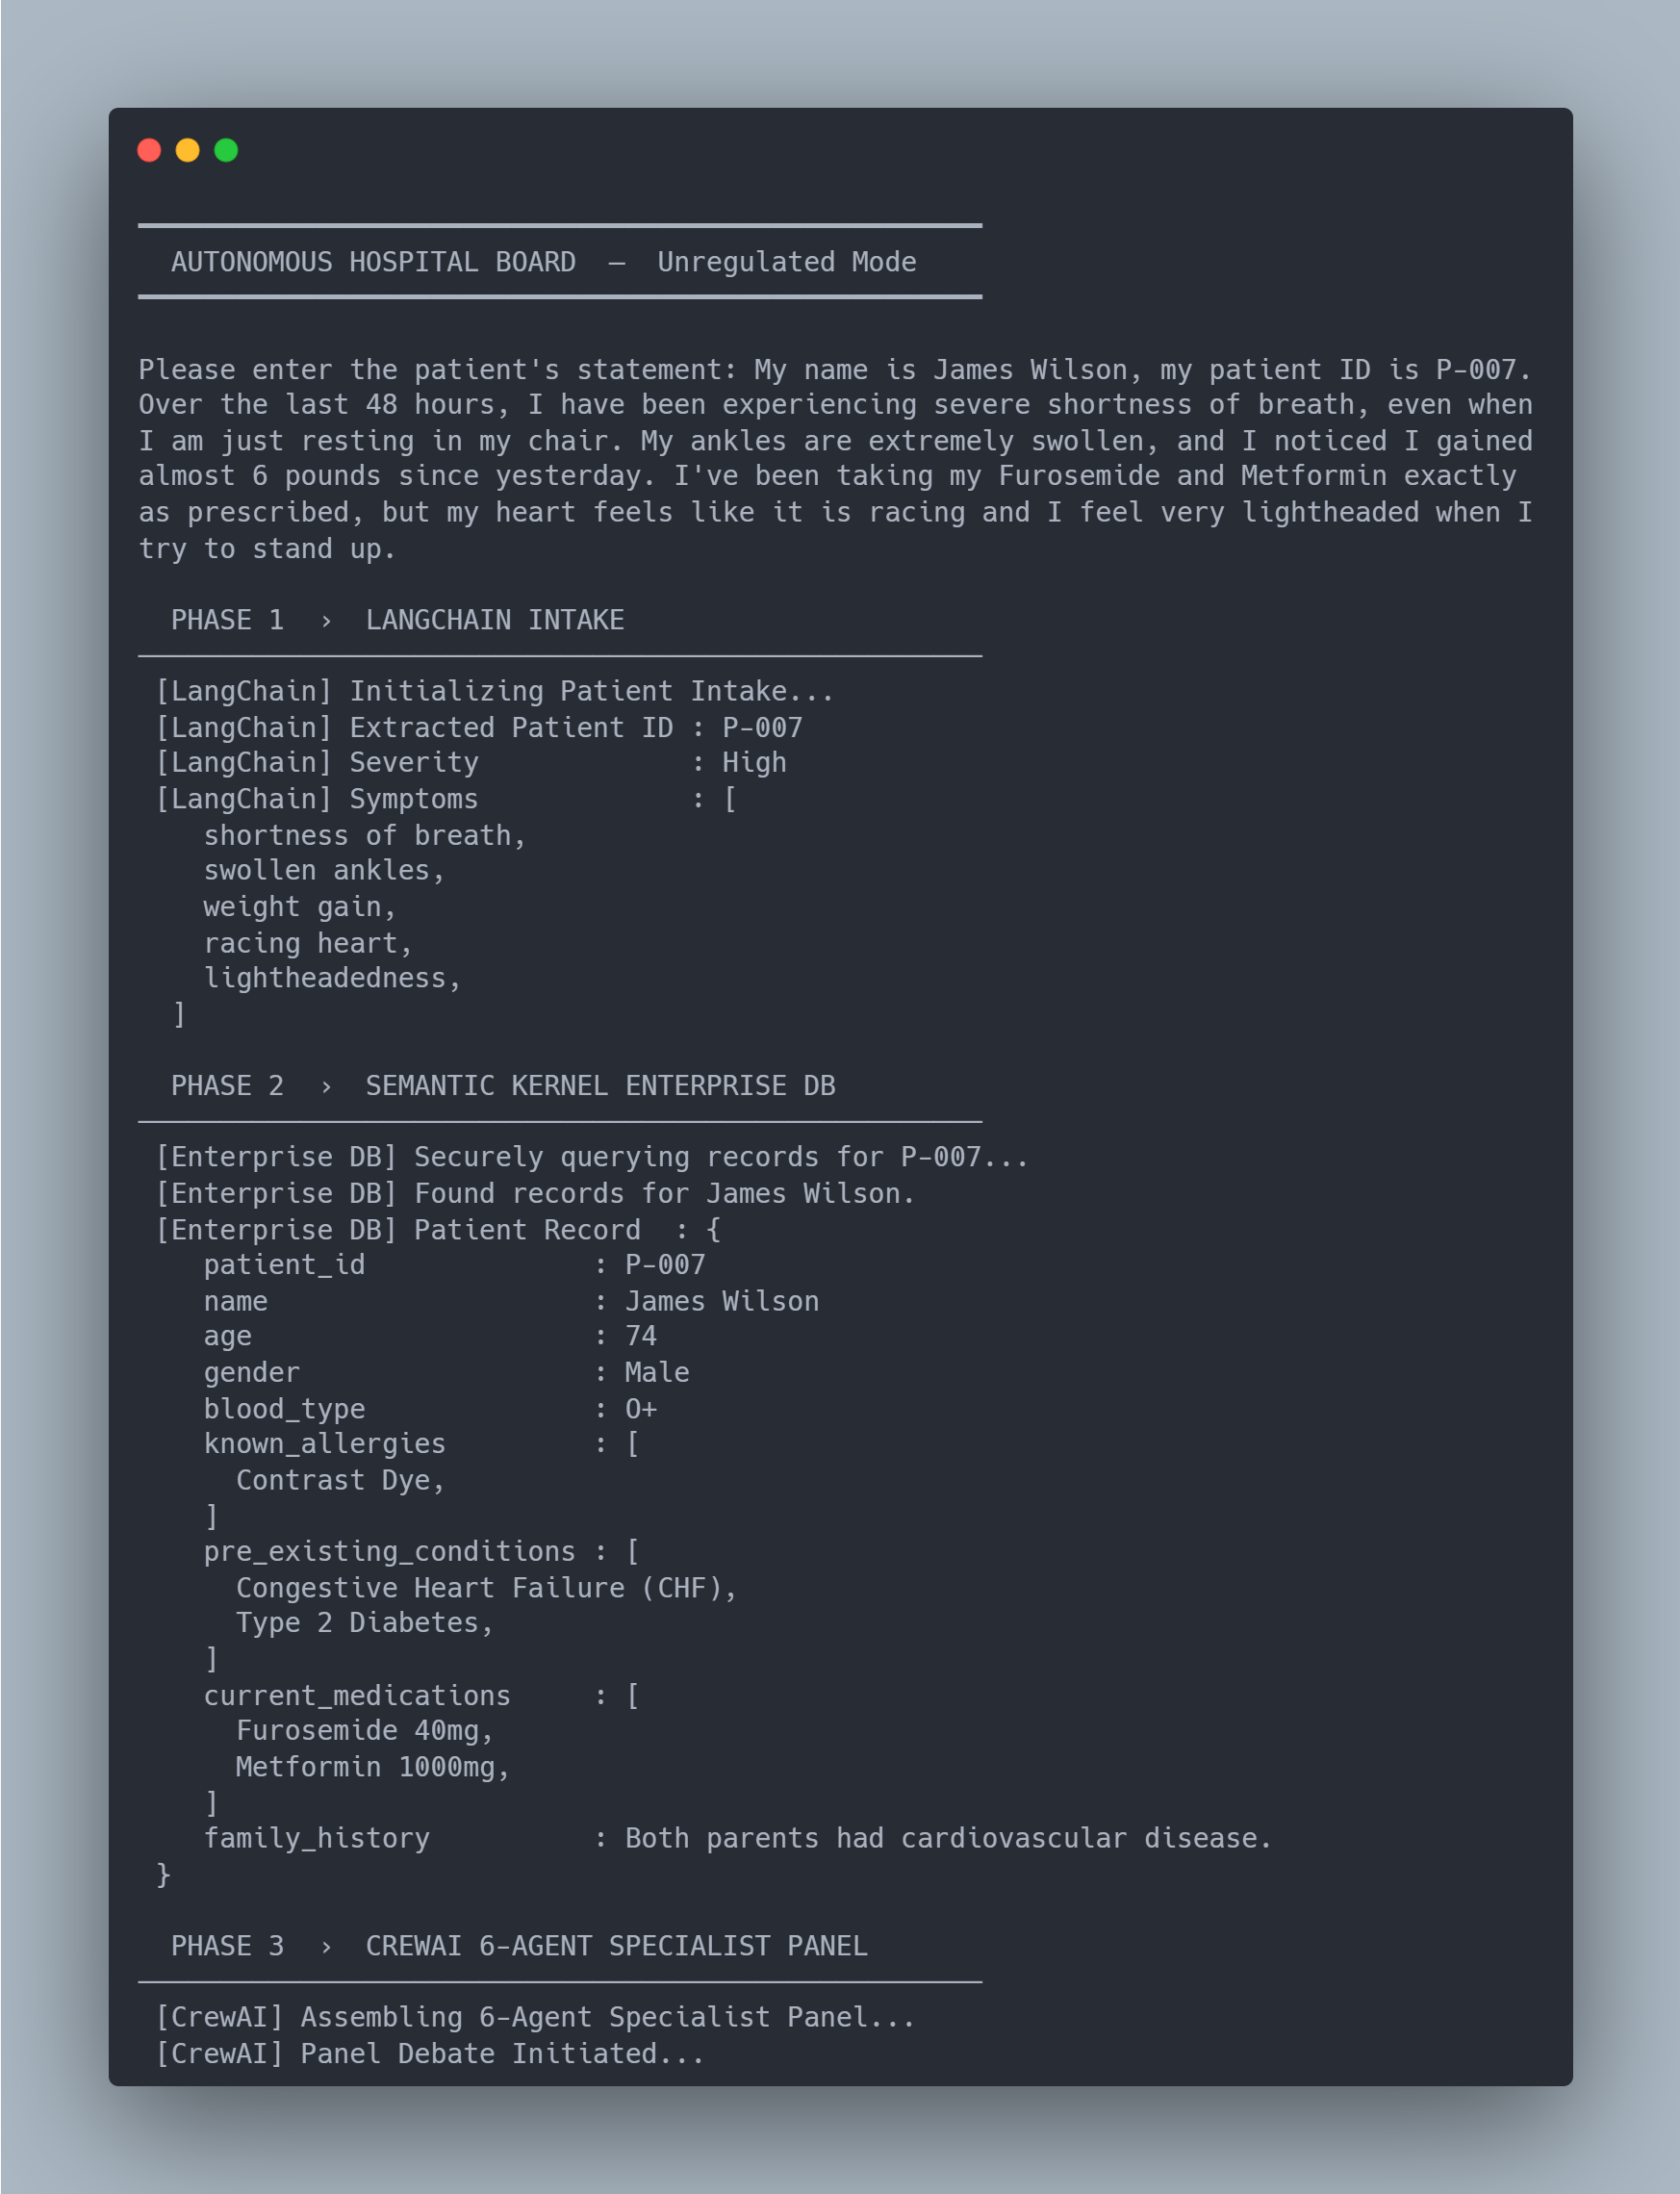
\includegraphics[width=0.88\textwidth]{carbon_before_p1.png}
\caption{Unregulated baseline run (no Attestix): Phase 1 LangChain intake and Phase 2 Enterprise DB with no security gates, no delegation verification, and no provenance logging.}
\label{fig:carbon_before_p1}
\end{figure}

A representative patient case (James Wilson, P-007, 74-year-old male presenting with acute decompensated congestive heart failure) was processed through the full regulated pipeline. The system correctly:
\begin{itemize}
    \item Extracted structured symptoms using LangChain (severity: High; shortness of breath, swollen ankles, weight gain)
    \item Retrieved patient history with allergy and medication records via UCAN-gated DB access
    \item Conducted a 6-specialist CrewAI debate identifying decompensated CHF as primary diagnosis
    \item Issued a final treatment plan including Furosemide dose adjustment and Contrast Dye allergy flag
    \item Generated a 4-entry Merkle provenance chain with all decisions hash-linked
\end{itemize}

\begin{figure}[H]
\centering
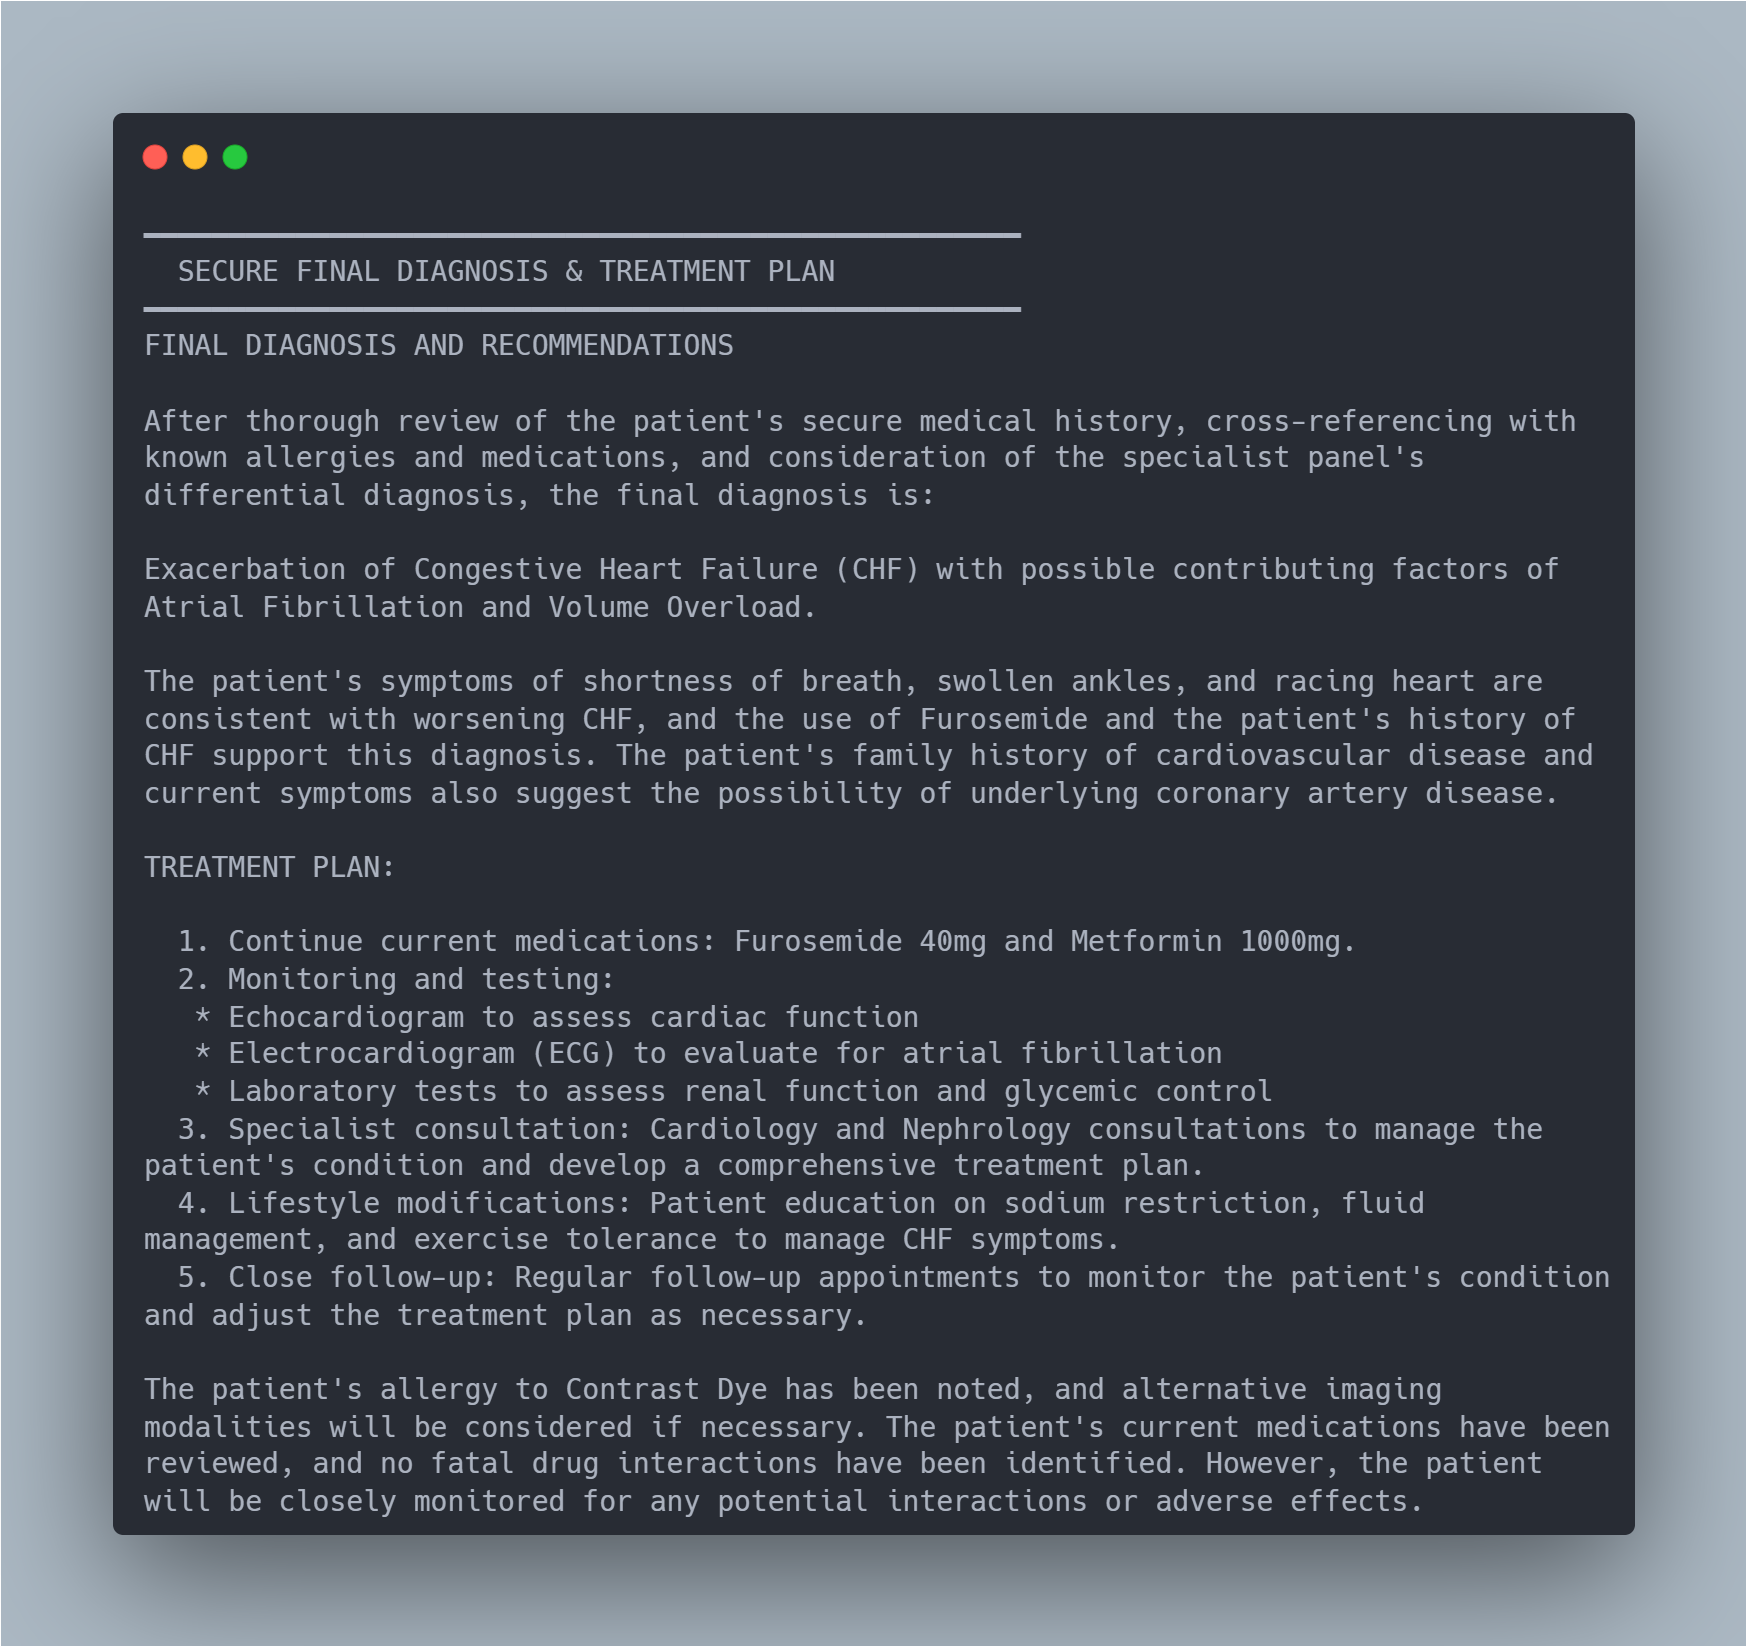
\includegraphics[width=0.88\textwidth]{carbon_regulated_result.png}
\caption{Hospital regulated run: secure final diagnosis and treatment plan issued by the Chief Medical Officer, with Contrast Dye allergy flagged and no fatal drug interactions identified.}
\label{fig:carbon_result}
\end{figure}

\begin{figure}[H]
\centering
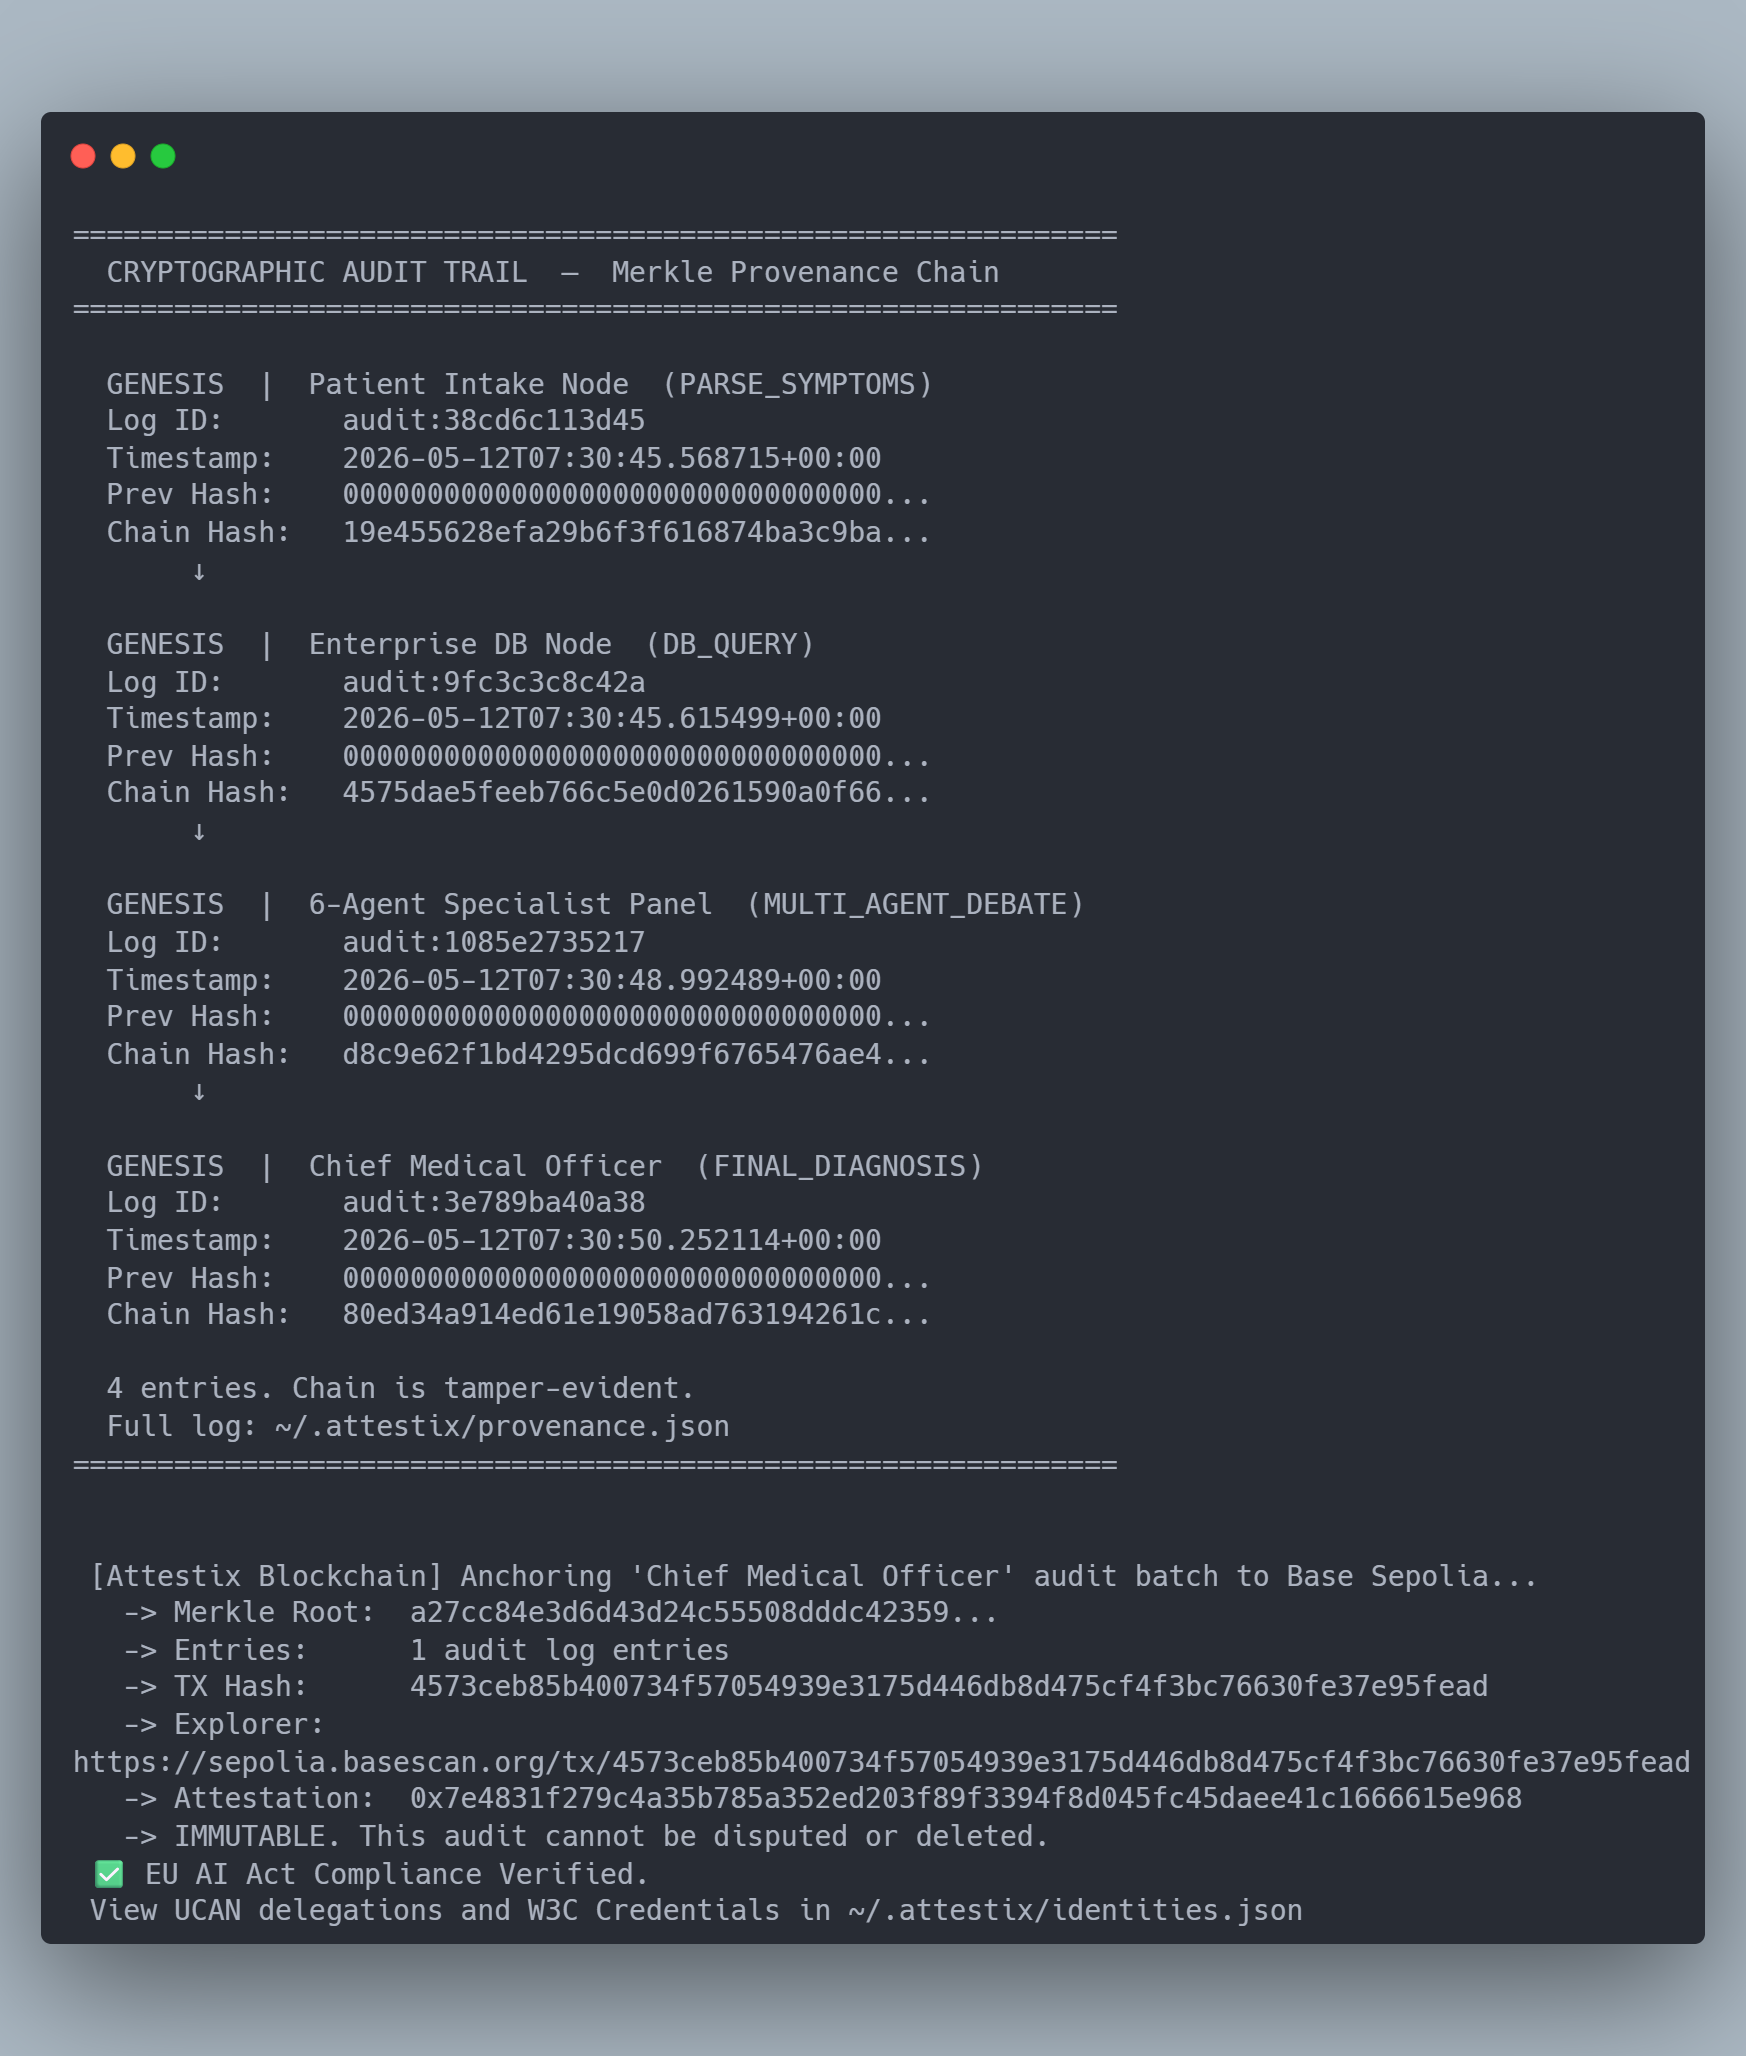
\includegraphics[width=0.88\textwidth]{carbon_merkle_blockchain.png}
\caption{Cryptographic audit trail (4-entry SHA-256 Merkle provenance chain) and Base Sepolia blockchain anchoring with TX hash, Merkle root, and EAS attestation UID.}
\label{fig:carbon_merkle}
\end{figure}

\begin{table}[H]
\centering
\caption{Hospital Merkle Provenance Chain --- Final Verified Run (2026-05-11)}
\label{tab:merkle_chain}
\begin{tabularx}{\textwidth}{|l|l|X|}
\hline
\textbf{Entry} & \textbf{Log ID} & \textbf{Chain Hash (SHA-256, truncated)} \\
\hline
Patient Intake Node & \texttt{audit:f301eb6ff424} & \texttt{62d70dfdba7d1803c755b208d996...} \\
Enterprise DB Node & \texttt{audit:bc595a3c972d} & \texttt{0aa53ab57c25d1b3f1b15b7ac998...} \\
6-Agent Specialist Panel & \texttt{audit:11e3946c2dd2} & \texttt{3d4011eb938aa771bd859d32d363...} \\
Chief Medical Officer & \texttt{audit:804133019f14} & \texttt{36bad1795d27b46fcef008153dcb...} \\
\hline
\end{tabularx}
\end{table}

\subsection{Blockchain Anchoring Results}

The final blockchain anchoring to Base Sepolia L2 via EAS was confirmed successful. The Merkle root of the Chief Medical Officer's audit batch was submitted as a permanent on-chain attestation.

\begin{figure}[H]
\centering
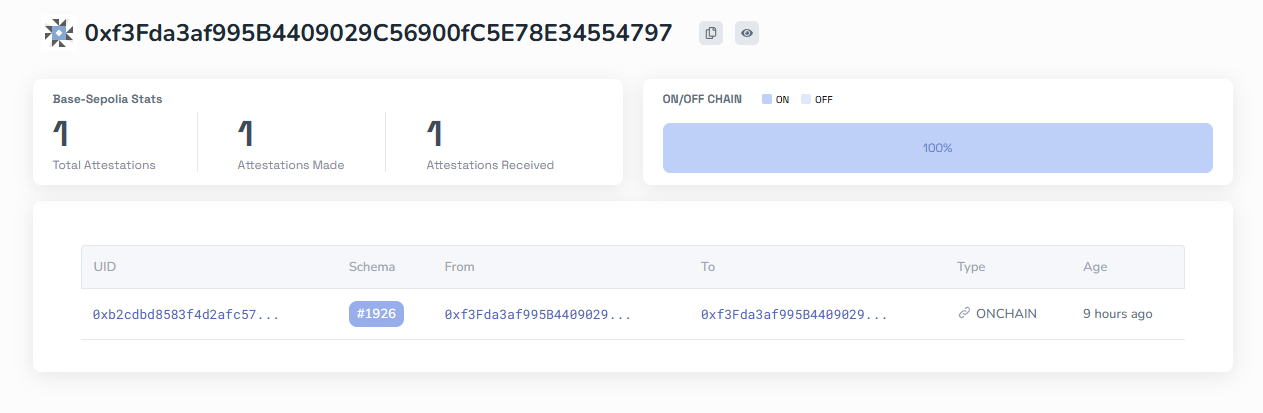
\includegraphics[width=0.92\textwidth]{easscan.png}
\caption{EAS attestation record on Base Sepolia confirming the hospital audit trail anchor (UID: \texttt{0xb2cdbd8583f4d2afc57...})}
\label{fig:easscan}
\end{figure}

\begin{figure}[H]
\centering
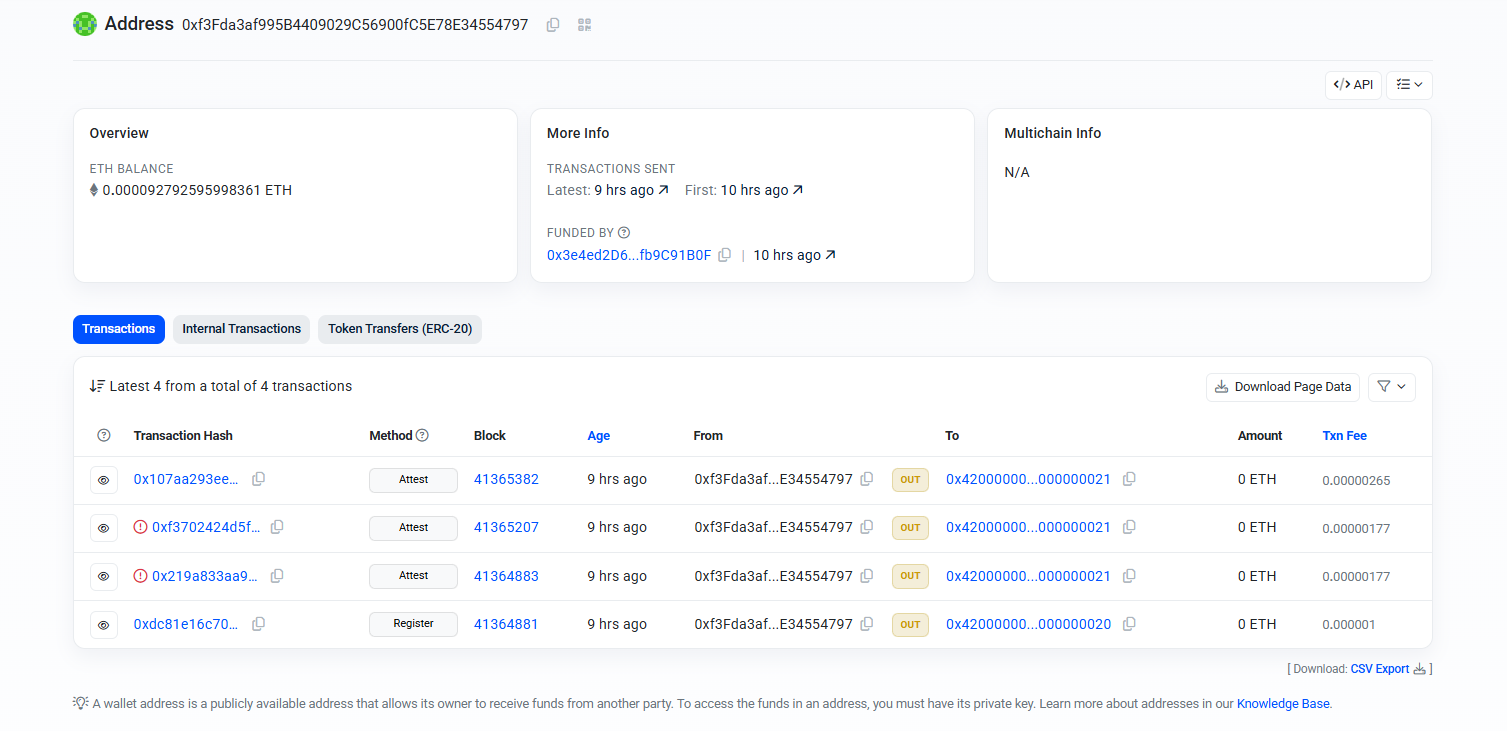
\includegraphics[width=0.92\textwidth]{History.png}
\caption{BaseScan wallet history: schema registration (block 41364881), two reverted attest transactions due to insufficient gas limit, and the final successful anchoring (block 41365382)}
\label{fig:basescan}
\end{figure}

\begin{table}[H]
\centering
\caption{Base Sepolia EAS Anchoring Record --- Confirmed Transaction}
\label{tab:blockchain_record}
\begin{tabularx}{\textwidth}{|l|X|}
\hline
\textbf{Field} & \textbf{Value} \\
\hline
Network & Base Sepolia (Chain ID: 84532) \\
Wallet Address & \texttt{0xf3Fda3af995B4409029C56900fC5E78E34554797} \\
Schema UID & \texttt{0x395d14d6af29e5b35fa76509e1293f05...} \\
Merkle Root & \texttt{79e1ea61c7c53e3b78804e2669749744...} \\
TX Hash & \texttt{107aa293eea834a69d3fc7ff8bc3202e...} \\
Attestation UID & \texttt{0xb2cdbd8583f4d2afc57d4a4859a89f3e...} \\
Explorer & \url{https://sepolia.basescan.org/tx/107aa293...} \\
Status & IMMUTABLE --- cannot be disputed or deleted \\
\hline
\end{tabularx}
\end{table}

\subsection{Threat Model Coverage}

\begin{table}[H]
\centering
\caption{Threat Model Coverage}
\label{tab:threat_model}
\begin{tabularx}{\textwidth}{|l|X|c|}
\hline
\textbf{Threat} & \textbf{Mitigation} & \textbf{Status} \\
\hline
Agent impersonation & Ed25519 DIDs, UAIT binding & $\checkmark$ Mitigated \\
Unauthorised data access & UCAN gate blocks unverified agents & $\checkmark$ Mitigated \\
Privilege escalation & UCAN capability attenuation enforced & $\checkmark$ Mitigated \\
Audit log tampering & SHA-256 Merkle chain & $\checkmark$ Mitigated \\
Unregistered agent execution & Conformity gatekeeper blocks & $\checkmark$ Mitigated \\
Token replay after expiry & JWT expiry verified & $\checkmark$ Mitigated \\
Revoked token use & JTI revocation list checked & $\checkmark$ Mitigated \\
Retroactive audit deletion & Merkle root anchored on-chain (EAS) & $\checkmark$ Mitigated \\
\hline
\end{tabularx}
\end{table}

\subsection{Summary}

The Attestix integration successfully satisfies all four requirements (R1--R4). Every agent decision is cryptographically accountable, unauthorized access is actively blocked, and the complete audit trail is preserved in a tamper-evident chain anchored permanently on Base Sepolia L2. The architecture performs consistently across all four domain simulations and five AI orchestration frameworks.
